\documentclass[border=3pt]{standalone}
% Preâmbulo compartilhado pelos diagramas TikZ da aula 12 (Mapeamento por Grade de Ocupação)
\usepackage[T1]{fontenc}
\usepackage[utf8]{inputenc}
\usepackage{lmodern}
\usepackage{amsmath}
\usepackage{xcolor}
\usepackage{tikz}
\usetikzlibrary{arrows.meta,angles,quotes,decorations.pathmorphing,calc,
                positioning,shapes.geometric,shapes.misc,backgrounds,fit,
                math}

% Paleta (mesma dos SVGs originais)
\definecolor{dblue}{HTML}{2A5B8C}
\definecolor{dorange}{HTML}{B3541E}
\definecolor{dgreen}{HTML}{4A7C59}
\definecolor{dred}{HTML}{9C4B4B}
\definecolor{dcream}{HTML}{F4F1EA}
\definecolor{dshade}{HTML}{DDD7C9}

% Função gaussiana (não normalizada por padrão de escala visual)
\pgfmathdeclarefunction{gauss}{3}{%
  \pgfmathparse{1/(#3*sqrt(2*pi))*exp(-((#1-#2)^2)/(2*#3^2))}%
}

% Estilos comuns (prefixo d... para não colidir com chaves internas do pgf)
\tikzset{
  >={Stealth[length=2mm]},
  dguide/.style={gray!55, dashed, line width=0.4pt},
  daxis/.style={gray!60, line width=0.7pt, ->},
  dbody/.style={fill=black!3, draw=black!80, line width=1pt},
  dacc/.style={draw=dblue, line width=1pt},
  dlbl/.style={black!55, font=\small},
  dsub/.style={black!45, font=\footnotesize},
  dstate/.style={circle, draw=black!80, fill=dcream, line width=1pt,
                 minimum size=17mm, font=\large, inner sep=1pt},
  dobs/.style={circle, draw=black!80, fill=dshade, line width=1pt,
               minimum size=14mm, font=\large, inner sep=1pt},
  dbox/.style={rounded corners=2pt, draw=black!80, fill=dcream, line width=1pt,
               align=center, inner sep=6pt},
  dop/.style={circle, draw=black!80, fill=white, line width=1pt,
              minimum size=6mm, inner sep=0pt, font=\small},
  dtrans/.style={->, dblue, line width=1pt},
  dmeas/.style={->, dorange, line width=1pt},
  dcurve/.style={line width=1pt, dblue},
  dcurveb/.style={line width=1.4pt, dorange},
}

\begin{document}
\hyphenpenalty=10000 \exhyphenpenalty=10000 \tolerance=9999 \emergencystretch=3em
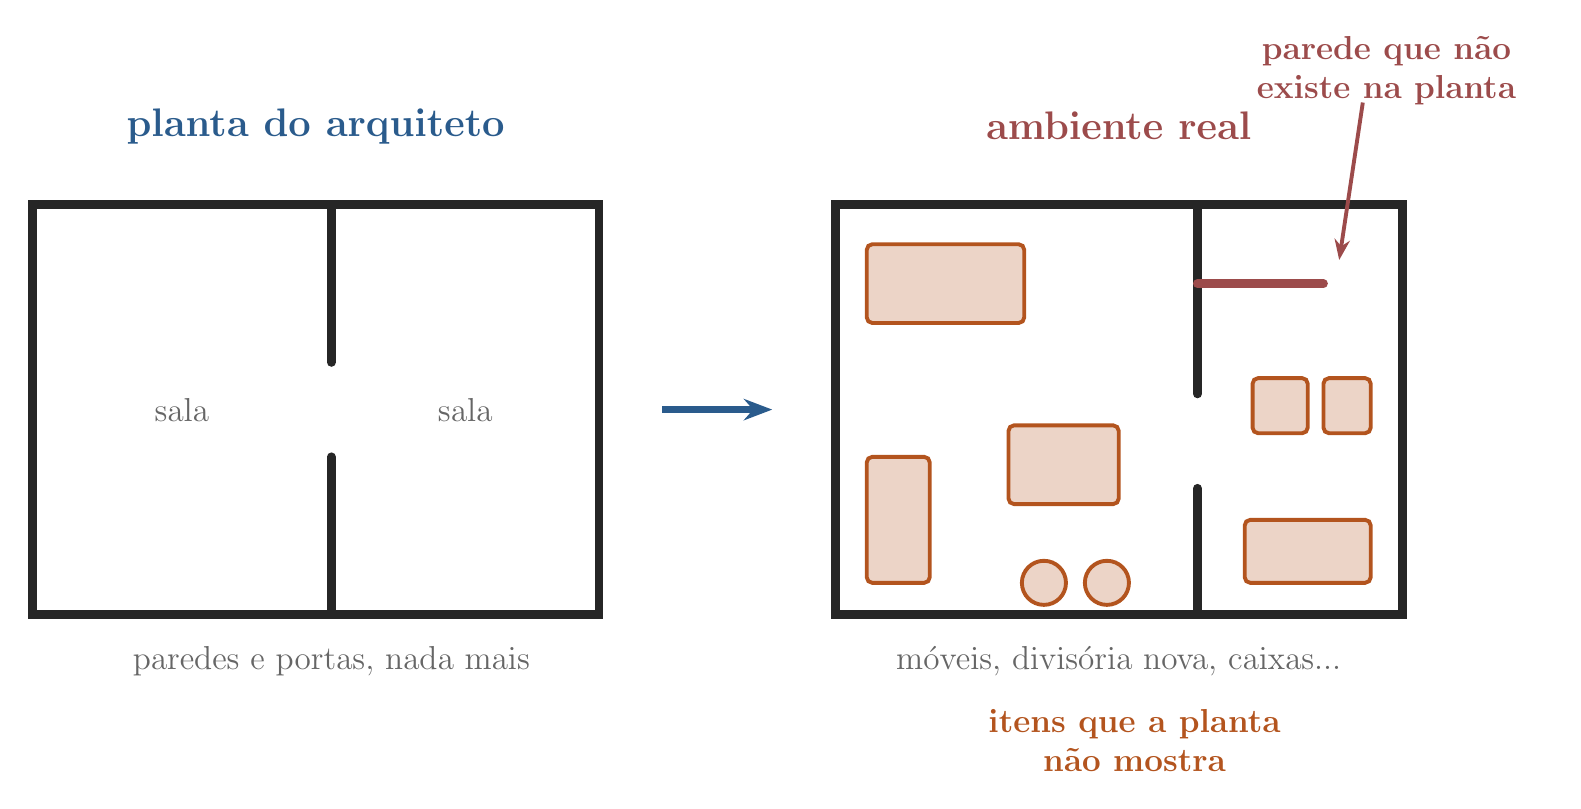
\begin{tikzpicture}[x=1cm,y=1cm]
  \tikzset{wall/.style={line width=3.2pt, black!85, line cap=round}, mov/.style={draw=dorange, fill=dorange!25, line width=1.4pt, rounded corners=2pt}}
  % ---- planta do arquiteto ----
  \node[font=\Large\bfseries, dblue] at (3.6,6.2) {planta do arquiteto};
  \draw[wall] (0,0) rectangle (7.2,5.2);
  \draw[wall] (3.8,0) -- (3.8,2.0); \draw[wall] (3.8,3.2) -- (3.8,5.2);
  \node[font=\large, black!60] at (1.9,2.6) {sala};
  \node[font=\large, black!60] at (5.5,2.6) {sala};
  \node[font=\large, black!60] at (3.8,-0.6) {paredes e portas, nada mais};
  % ---- seta ----
  \draw[dtrans, line width=2.6pt, -{Stealth[length=3.6mm]}] (8.0,2.6) -- (9.4,2.6);
  % ---- ambiente real ----
  \begin{scope}[shift={(10.2,0)}]
    \node[font=\Large\bfseries, dred] at (3.6,6.2) {ambiente real};
    \draw[wall] (0,0) rectangle (7.2,5.2);
    \draw[wall] (4.6,0) -- (4.6,1.6); \draw[wall] (4.6,2.8) -- (4.6,5.2);
    \draw[wall, dred] (4.6,4.2) -- (6.2,4.2);
    \draw[mov] (0.4,3.7) rectangle (2.4,4.7);
    \draw[mov] (0.4,0.4) rectangle (1.2,2.0);
    \draw[mov] (2.2,1.4) rectangle (3.6,2.4);
    \foreach \x in {0.75,1.55} {\draw[mov] (\x+1.9,0.4) circle (0.28);}
    \draw[mov] (5.2,0.4) rectangle (6.8,1.2);
    \draw[mov] (5.3,2.3) rectangle (6.0,3.0);
    \draw[mov] (6.2,2.3) rectangle (6.8,3.0);
    \node[font=\large, dorange, anchor=east] at (-0.1,6.2) {};
    \node[font=\large, black!60] at (3.6,-0.6) {móveis, divisória nova, caixas...};
  \end{scope}
  \node[font=\large\bfseries, dorange, text width=4cm, align=center] at (14.0,-1.6) {itens que a planta \textbf{não mostra}};
  \node[font=\large\bfseries, dred, text width=4cm, align=center] at (17.2,6.9) {parede que \textbf{não existe} na planta};
  \draw[dred, line width=1.4pt, -{Stealth[length=2.6mm]}] (16.9,6.5) -- (16.6,4.5);
\end{tikzpicture}
\end{document}
